\chapter{Conception détaillée du système}
\par  Dans ce chapitre, nous entamerons la phase de conception dans le but de présenter une
solution applicative répondant aux besoins retenus. Dans cette optique, l'architecture et les diagrammes de séquence sont définis. 


\clearpage
\section{Introduction}
Le chapitre de la conception détaillée du système joue un rôle crucial dans le développement d'un projet de banque en ligne. Il s'agit d'une phase clé où nous passons de la phase de conception générale à une représentation plus spécifique et détaillée de l'architecture, des fonctionnalités et du comportement de notre application.\\

Dans ce chapitre, nous allons explorer en profondeur la conception de notre système de banque en ligne, en utilisant diverses techniques et outils de modélisation pour représenter les différents aspects du système. Nous allons examiner les principaux éléments de conception tels que l'architecture globale, les composants clés, les interactions entre les modules, ainsi que les fonctionnalités spécifiques.\\

L'objectif de cette phase de conception détaillée est de créer une base solide pour le développement de notre application. Nous allons utiliser des techniques éprouvées, telles que le diagramme de classe, les diagrammes de séquences, l'architecture en couches, les modèles de conception, et d'autres méthodes de modélisation pour représenter les différentes parties du système.

\section{Architecture logique d'UNIBANK}
Ce projet est réalisé en collaboration avec l'équipe Unibank, qui joue un rôle clé en tant que moteur BACKEND pour les différents projets au sein de la SG ABS. Unibank est une plateforme d'Open Banking innovante qui répond aux besoins digitaux des filiales de la région AFS. L'Open Banking est une initiative réglementaire qui exige des banques d'ouvrir leurs API à des services tiers, permettant ainsi le partage de données financières des clients de manière conforme et standardisée. Il fournit des orientations pour moderniser les approches bancaires et améliorer le service client.\\

Cependant, chaque banque peut adopter une approche personnalisée pour mettre en œuvre des projets adaptés à son activité. C'est dans ce contexte que la Digital Factory a développé la plateforme digitale UNIBANK. Cette plateforme permet de construire rapidement des solutions qui consomment des services CBS (ou autres) en simplifiant la complexité de ces différents services.\\

La structure de la plateforme UNIBANK est illustrée dans la figure suivante :

\begin{figure}[!h]
    \centering %
        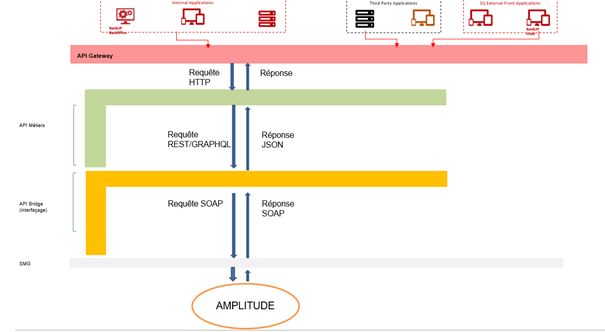
\includegraphics[width=16cm]{images/conception/architectureUNIBANK.png}
    \caption{Rôle des APIs UNIBANK dans le cadre du programme Bank-UP}
\end{figure}
\newpage

La plateforme UNIBANK est composée de trois couches distinctes :

\begin{itemize}
    \item[•] \textbf{L'API Bridge} assure une communication sécurisée avec les systèmes d'informations externes tels qu'Amplitude et Infobip, en utilisant des connecteurs. Son rôle est d'intégrer, de mapper et de traduire les données entre les APIs UNIBANK et ces systèmes externes.
    \item[•] \textbf{Les APIs métier} transforment et exploitent les données provenant du bridge ou des systèmes externes en appliquant des règles de gestion métier. Elles répondent ainsi à des besoins spécifiques des applications clientes, tels que l'affichage des comptes ou l'exécution de virements.
    \item[•] \textbf{ Les Gateways} sont des composants supplémentaires qui garantissent un accès sécurisé aux APIs UNIBANK en utilisant un mode d'authentification. Ils exposent les données provenant des APIs UNIBANK aux applications clientes.
\end{itemize}

\section{Architecture technique d'UNIBANK}
\textbf{\large{Architecture Hexagonal}\\}

Dans l'architecture technique d'UNIBANK, l'approche hexagonale a été adoptée pour préserver la logique métier, qui représente la plus grande valeur ajoutée de l'application. Cette architecture se compose de trois principales parties : le domaine métier (User Side), l'application (Business Logic) et l'infrastructure (Server Side).

\begin{figure}[!h]
    \centering %
        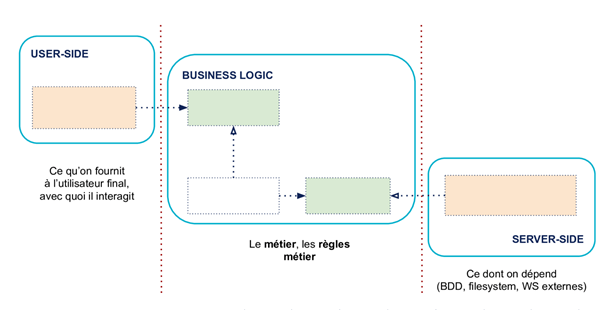
\includegraphics[width=16cm]{images/conception/hexagonal.png}
    \caption{Couches de l’architecture Hexagonale}
\end{figure}

\begin{itemize}
    \item[•] \textbf{Le domaine métier (User Side)} est le côté par lequel les utilisateurs ou les programmes extérieurs interagissent avec l'application. On y trouve le code qui gère ces interactions, tels que le code d'interface utilisateur, les routes HTTP pour une API et les sérialisations en JSON destinées à d'autres programmes qui consomment l'application.
    \item[•] \textbf{L'application (Business Logic)} est la partie centrale de l'architecture où se trouve toute la logique métier. On y retrouve le vocabulaire métier et la logique purement métier, qui résolvent le problème concret auquel l'application est dédiée. Cette partie contient la richesse et la spécificité de l'application. L'objectif est que même un expert du métier, sans compétences en développement, puisse lire le code de cette partie et identifier les incohérences éventuelles.
    \item[•] \textbf{L'infrastructure (Server Side)} regroupe les composants nécessaires au bon fonctionnement de l'application. On y trouve le code qui interagit avec la base de données, effectue des appels système de fichiers ou gère des appels HTTP vers d'autres applications. Cette partie est responsable de la mise en place de l'infrastructure technique nécessaire à l'exécution de l'application.
\end{itemize}

Au sein de la DiFa, UNIBANK a adapté cette architecture pour répondre à ses besoins techniques et fonctionnels. Toutefois, en raison de la dépendance du Bridge (connecteur externe) à un CBS externe, quelques modifications ont été apportées à l'architecture. L'accent a été mis sur deux couches principales :

\begin{itemize}
    \item[1-] \textbf{unibank-domain (Domain layer) :} Cette couche contient deux sous-projets Java :
    \begin{itemize}
        \item[-] \textbf{Platform model :} Il s'agit du socle technique du domaine, qui comprend les annotations, la gestion des permissions, la documentation, etc.
        \item[-] \textbf{Core domain :}  Ce sous-projet contient des classes Java qui représentent des besoins anticipés de l'application. Il regroupe la logique métier de la banque, divisée en trois packages :
        \begin{itemize}
            \item[•] \textbf{Base :} Ce package contient les classes POJO nécessaires pour créer une requête/réponse afin de satisfaire un besoin anticipé.
            \item[•] \textbf{Business :} Ce package gère la gestion des administrateurs et des utilisateurs.
            \item[•] \textbf{Providers :} Ce package représente la majeure partie du travail réalisé. Il contient des classes POJO utilisées par presque tous les connecteurs.
        \end{itemize}
    \end{itemize}
    \item[2-] \textbf{unibank-bridge (Application Layer)} Cette couche contient un ensemble de connecteurs, un module de configuration et un module d'exposition jouant le rôle d'adaptateur :
    \begin{itemize}
        \item[-] \textbf{Les connecteurs :} Ces modules exposent des APIs répondant à des besoins souvent techniques.
        \item[-] \textbf{Module de configuration :} Ce module gère la configuration des filiales et des connecteurs. Chaque environnement de développement dispose de sa propre configuration, soit par le biais d'un fichier de configuration, soit par l'utilisation de Vault.
        \item[-] \textbf{Module d'exposition (Adaptateur) :} Pour assurer un couplage faible, unibank a proposé ce module pour gérer la partie de la création des Beans java. Dans ce module et en se basant sur le module de configuration on peut exposer nos APIs pour n’importe
        quel connecteur.
    \end{itemize}
\end{itemize}

\begin{figure}[!h]
    \centering %
        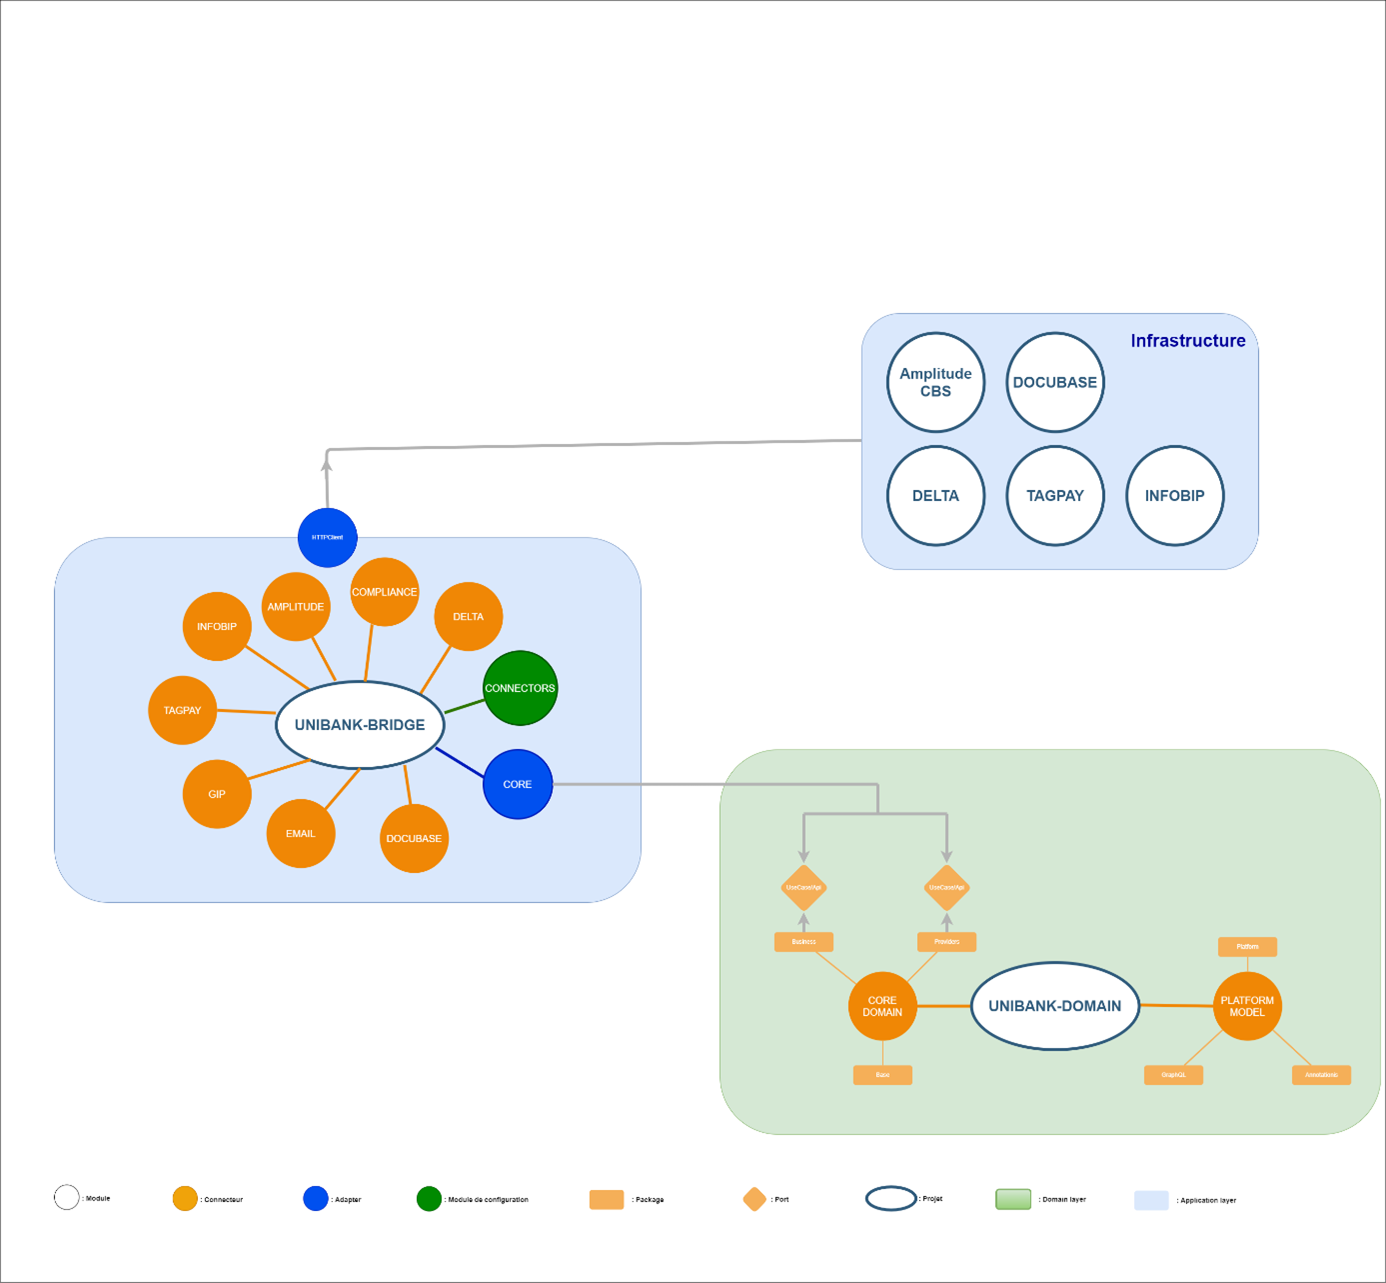
\includegraphics[width=16cm]{images/conception/architectureTechnique.png}
    \caption{Architecture technique d’UNIBANK}
\end{figure}
\newpage

\section{Technique d'Authentification/Authorisation}
Une fois que le token est généré par WSO2, il doit passer par une couche de vérification pour s'assurer de sa validité, de sa non-expiration et du type d'utilisateur qui l'utilise. Pour cela, nous utilisons un package appelé Jwt dans unibank-platform. Voici un résumé du processus de vérification des tokens :
\begin{enumerate}
    \item L'utilisateur envoie le token dans l'en-tête de la requête HTTP.
    \item En utilisant un filtre HTTP implémenté dans unibank-platform et en appliquant la méthode parseToken, nous pouvons extraire les informations de l'utilisateur :
    
    \begin{figure}[!h]
        \centering %
            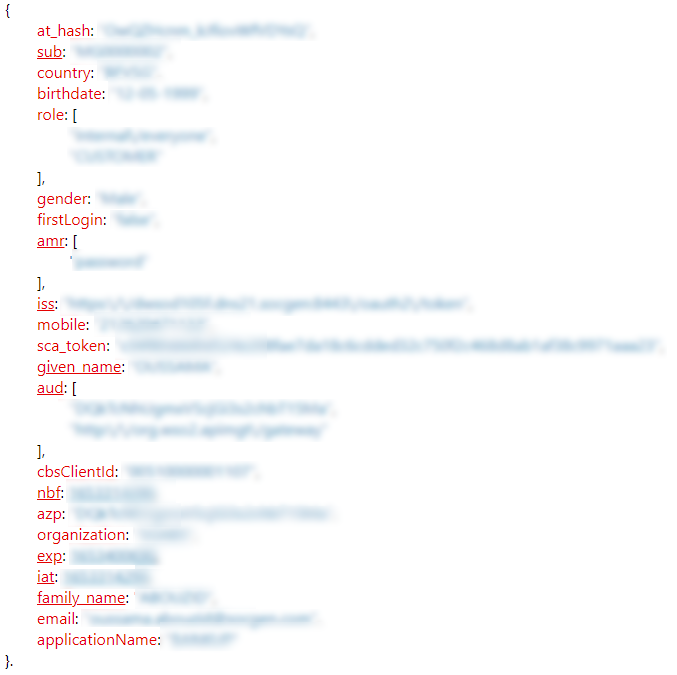
\includegraphics[width=16cm]{images/conception/exempleDeDonnees.png}
        \caption{Exemple de données d’un utilisateur en se basant sur son Token}
    \end{figure}
    \newpage

    \item La méthode parseToken permet de déchiffrer le token en utilisant l'algorithme RS256, que nous détaillerons par la suite.
    \item Après le déchiffrement du token, nous pouvons identifier l'utilisateur qui souhaite consommer l'API ainsi que ses droits.\\
\end{enumerate}

\textbf{\large{L'algorithme RS256}\\}

L'algorithme RS256 est un algorithme de cryptographie asymétrique. Cela signifie que l'émetteur du token possède une clé privée qu'il utilise pour générer la signature, tandis que le consommateur du JWT utilise une clé publique pour valider la signature. Cet algorithme est couramment utilisé pour échanger des données confidentielles sur un réseau.

\begin{figure}[!h]
    \centering %
        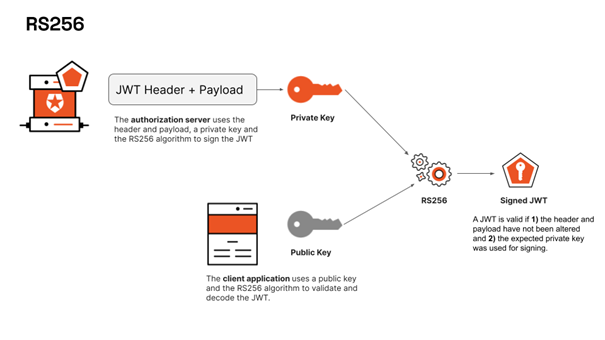
\includegraphics[width=16cm]{images/conception/algorithme.png}
    \caption{Principe d’algorithme RS256}
\end{figure}

Cet algorithme est basé sur une problématique mathématique assez célèbre, en effet supposant qu'on a p * q = n avec $n \in Z $ et p et q sont des nombres premiers, si nous savons p et q en peut déduire n, mais le contraire est très difficile.


\section{Connecteurs externes}
\textbf{\large{AMPLITUDE}\\}

\par Amplitude est un système bancaire de base (CBS) utilisé pour prendre en charge les transactions courantes d'un établissement bancaire. Les fonctionnalités bancaires de base varient en fonction du type spécifique d'établissement. Par exemple, les banques de détail ciblent les clients particuliers, tandis que les banques d'investissement traitent principalement des transactions entre institutions financières. Les systèmes bancaires de base sont souvent spécialisés dans un type spécifique d'opérations bancaires, tandis que les systèmes bancaires universels sont conçus pour prendre en charge plusieurs types de fonctions bancaires.\\

Pour répondre à ses besoins métiers, la Digital Factory utilise le CBS de Sopra, qui propose une solution robuste appelée Amplitude.\\

\textbf{\large{INFOBIP}\\}

Infobip est une entreprise leader dans le domaine des solutions de communication cloud et de messagerie omnicanal. Leur plateforme permet aux entreprises d'envoyer des messages SMS, des messages vocaux, des e-mails et d'autres types de notifications à leurs clients dans le monde entier. Infobip offre également une gamme de services de messagerie instantanée, tels que WhatsApp, Facebook Messenger et Viber, qui facilitent la communication directe avec les clients via les applications de messagerie les plus populaires.\\

\textbf{\large{EMAIL}\\}

Le courrier électronique repose sur le concept client/serveur, ce qui implique l'utilisation de deux composants : le client de messagerie (Mail User Agent : MUA), tel que Outlook, Messenger, Eudora, et le serveur de messagerie (Mail Transport Agent : MTA), tel que SendMail. Les clients de messagerie s'appuient sur un serveur de messagerie pour recevoir et envoyer des messages.\\

Dans le contexte bancaire, l'envoi d'e-mails via les API backend revêt une grande importance, car cela permet de sécuriser le traitement des données clients et de notifier en temps réel les opérations effectuées sur leur compte. Le connecteur EMAIL facilite ainsi l'envoi de courriers électroniques aux clients après une ou plusieurs opérations bancaires.

\section{Architecture Monorepo de la partie Front-end}
Dans le projet de banque en ligne, l'architecture monorepo a été choisie pour regrouper les différentes applications, à savoir le développement web, mobile et une autre application spécifique. Cette approche consiste à centraliser l'ensemble du code source dans un seul référentiel, offrant ainsi une vision unifiée de toutes les applications.\\

L'adoption de l'architecture monorepo présente plusieurs avantages. Tout d'abord, elle favorise la collaboration entre les équipes de développement en simplifiant le partage de code entre les différentes plates-formes. Les développeurs peuvent travailler plus efficacement en réutilisant les composants et les fonctionnalités communes, ce qui accélère le processus de développement et garantit une cohérence globale.\\

De plus, l'architecture monorepo facilite la maintenance et les mises à jour du système. Les modifications apportées à une partie de l'application peuvent être rapidement propagées à l'ensemble du système, ce qui réduit les risques d'incohérence et améliore la stabilité globale de l'application.\\

En comparaison, l'approche multi-repo, qui consiste à maintenir des référentiels distincts pour chaque application ou composant, présente une séparation plus stricte entre les différents éléments. Bien qu'elle puisse offrir une isolation plus granulaire et faciliter la gestion indépendante des applications, elle peut également entraîner une duplication de code et rendre le partage de fonctionnalités plus complexe.

\begin{figure}[!h]
    \centering %
        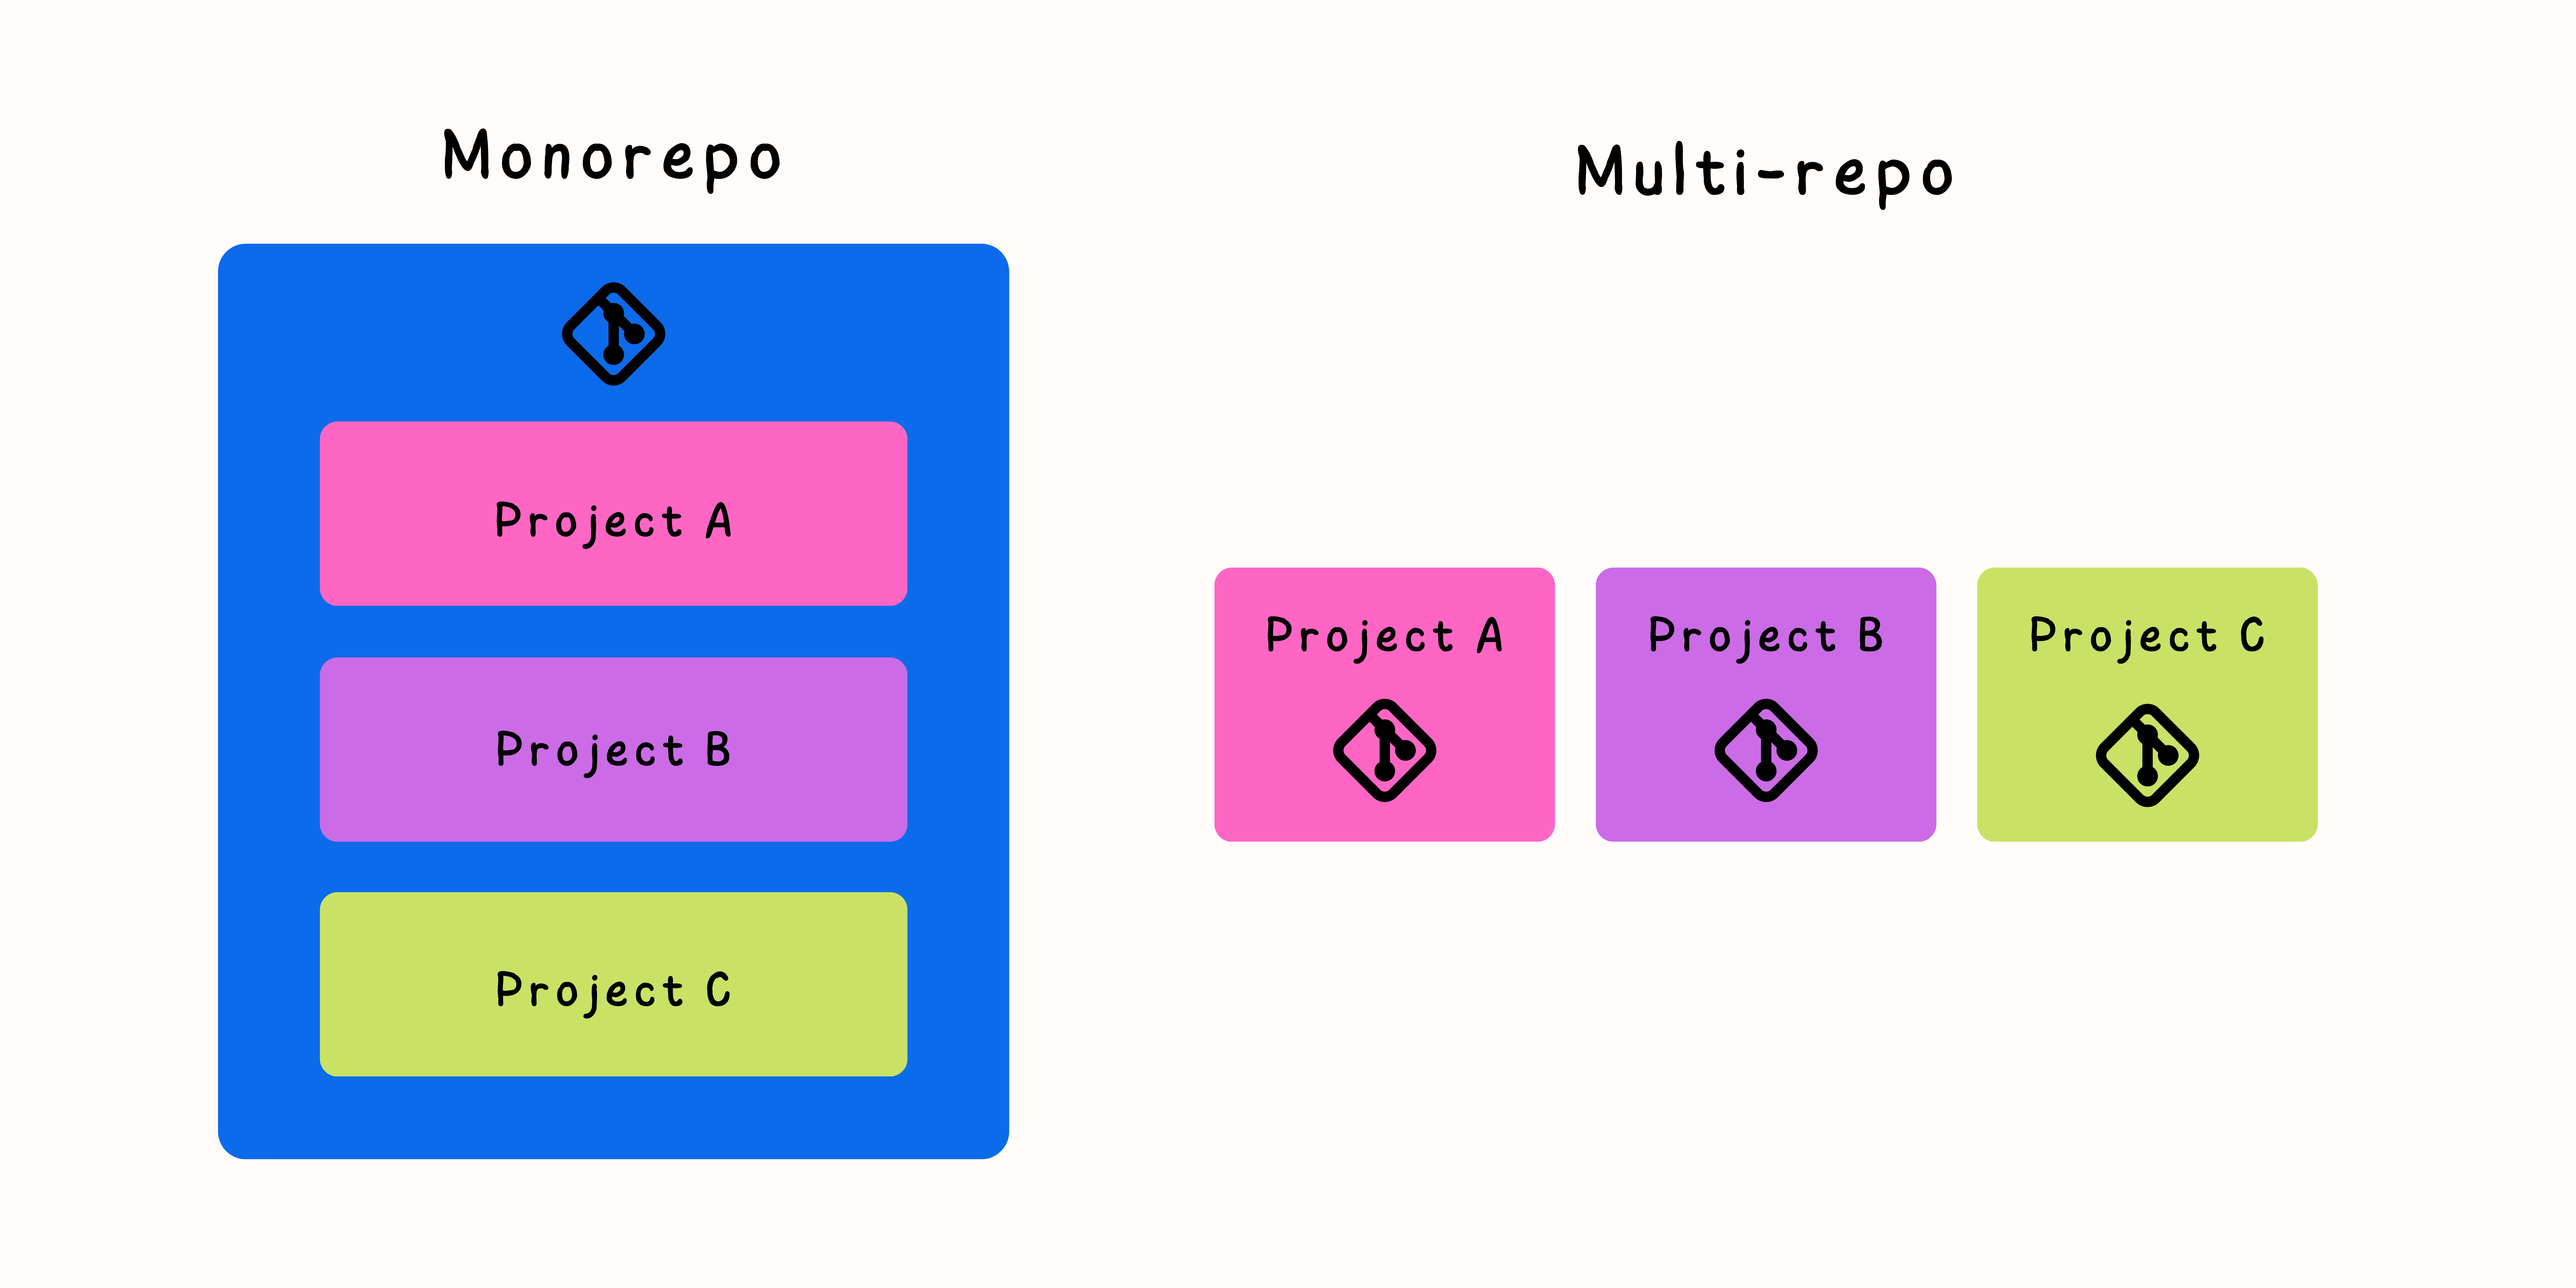
\includegraphics[width=16cm]{images/conception/monoRepo.png}
    \caption{Comparaison entre l’architecture monorepo et multi-repo}
\end{figure}

Dans l'architecture détaillée du Front-End de l'application SG CONNECT, représentée dans la figure suivante :
\begin{figure}[!h]
    \centering %
        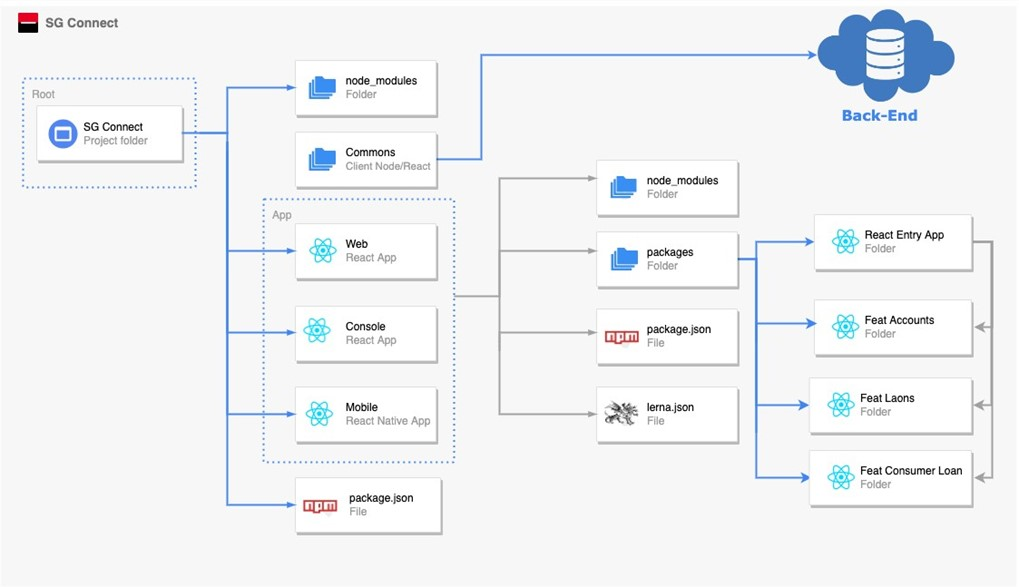
\includegraphics[width=14cm]{images/conception/architectureFRONT.jpg}
    \caption{Architecture Front-End du SG CONNECT}
\end{figure}

nous avons trois applications FRONT regroupées dans un monorepo. Ces applications servent les clients de la banque de détail des filiales AFS. Les trois applications sont les suivantes :

\begin{itemize}
    \item[•] Une application mobile compatible avec les plateformes Android et iOS.
    \item[•] Une application web pour une expérience utilisateur conviviale via les navigateurs.
    \item[•] Une application web console backoffice destinée aux gestionnaires afin de consulter les demandes des clients et gérer les opérations internes.
\end{itemize}

Cette architecture monorepo permet de maximiser l'efficacité de développement tout en assurant la cohérence et la stabilité de l'ensemble du système. Les équipes de développement peuvent travailler de manière collaborative, partager efficacement le code et garantir une expérience utilisateur homogène sur les différentes plates-formes.

\section{Approche Multitenant}
L'approche multitenant a été choisie afin d'éviter la duplication de code spécifique à chaque entité et de gérer efficacement les multiples clients ou filiales au sein d'une seule instance de l'application. Cette approche permet de maintenir l'isolation des données, des configurations et des personnalisations propres à chaque locataire (tenant). Une alternative à cette approche est le modèle \textbf{single tenant}, où chaque filiale dispose d'une instance dédiée de l'application avec ses propres configurations.\\

Pour simplifier la gestion des filiales, un fichier de configuration spécifique à chaque tenant, appelé \textbf{tenantconfig}, est utilisé dans le cadre de l'approche multitenant. Ce fichier contient les paramètres, les valeurs et les personnalisations propres à chaque filiale. Il permet de définir des fonctionnalités spécifiques activées ou désactivées, des règles d'accès, des paramètres de personnalisation de l'interface utilisateur et d'autres configurations uniques pour chaque entité.\\

Comparativement, le modèle \textbf{single tenant} nécessiterait la création et la maintenance de différentes instances de l'application pour chaque filiale, ce qui entraînerait une complexité accrue et une duplication des efforts de développement et de maintenance. En utilisant l'approche multitenant avec un fichier \textbf{tenantconfig}, il est possible de centraliser la gestion des différentes filiales tout en permettant une personnalisation spécifique à chaque entité. Cela favorise une approche plus efficace et évolutive pour le développement et la maintenance de l'application dans un environnement multitenant.
\begin{figure}[!h]
    \centering %
        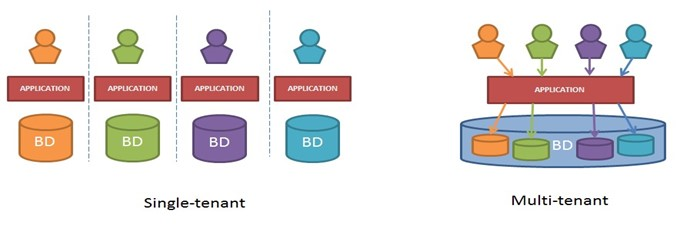
\includegraphics[width=14cm]{images/conception/teant.jpg}
    \caption{Comparaison entre l’approche single tenant et multitenant}
\end{figure}

\section{Feature Flagging}
Le \textbf{Feature Flagging} est une approche qui permet de gérer les fonctionnalités de manière flexible. Les fonctionnalités peuvent être activées ou désactivées dynamiquement en fonction des besoins et des paramètres définis. Cette approche nous offre la possibilité de tester et de déployer progressivement de nouvelles fonctionnalités, ce qui réduit les risques potentiels et garantit une meilleure qualité et stabilité du système.\\

En utilisant le "Feature Flagging", nous pouvons limiter l'impact des changements en activant les fonctionnalités uniquement pour un groupe restreint d'utilisateurs ou pour des tests internes, avant de les rendre accessibles à tous. Cela nous permet de contrôler l'exposition des nouvelles fonctionnalités et de recueillir des commentaires et des données de manière contrôlée.\\

De plus, le \textbf{Feature Flagging} offre une gestion facile des fonctionnalités en fonction des besoins spécifiques des filiales. En activant ou désactivant les drapeaux appropriés, nous pouvons personnaliser l'expérience utilisateur pour chaque filiale en leur offrant des fonctionnalités spécifiques ou en adaptant des fonctionnalités existantes selon leurs exigences. Cela nous permet de répondre aux besoins uniques de chaque filiale sans nécessiter des développements séparés pour chaque cas.
\begin{figure}[!h]
    \centering %
        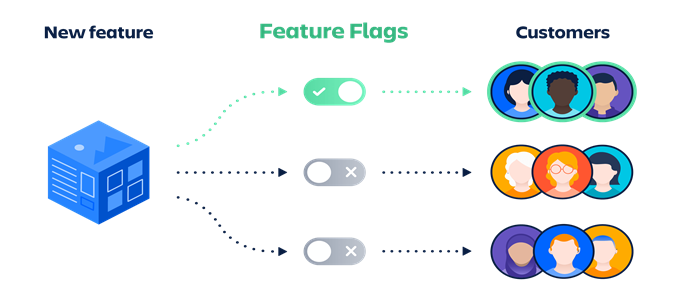
\includegraphics[width=14cm]{images/conception/flagging.png}
    \caption{Feature flagging}
\end{figure}

\section{Diagramme de classes}
Le diagramme de classes montre la structure interne du système. Il permet de fournir une
représentation abstraite des objets du système, qui vont interagir ensemble pour réaliser les cas
d’utilisation, il faut noter que ce diagramme ne présente pas toutes les classess du système, mais il présente les classes utilisées dans le projet.\\
\begin{figure}[!h]
    \centering %
        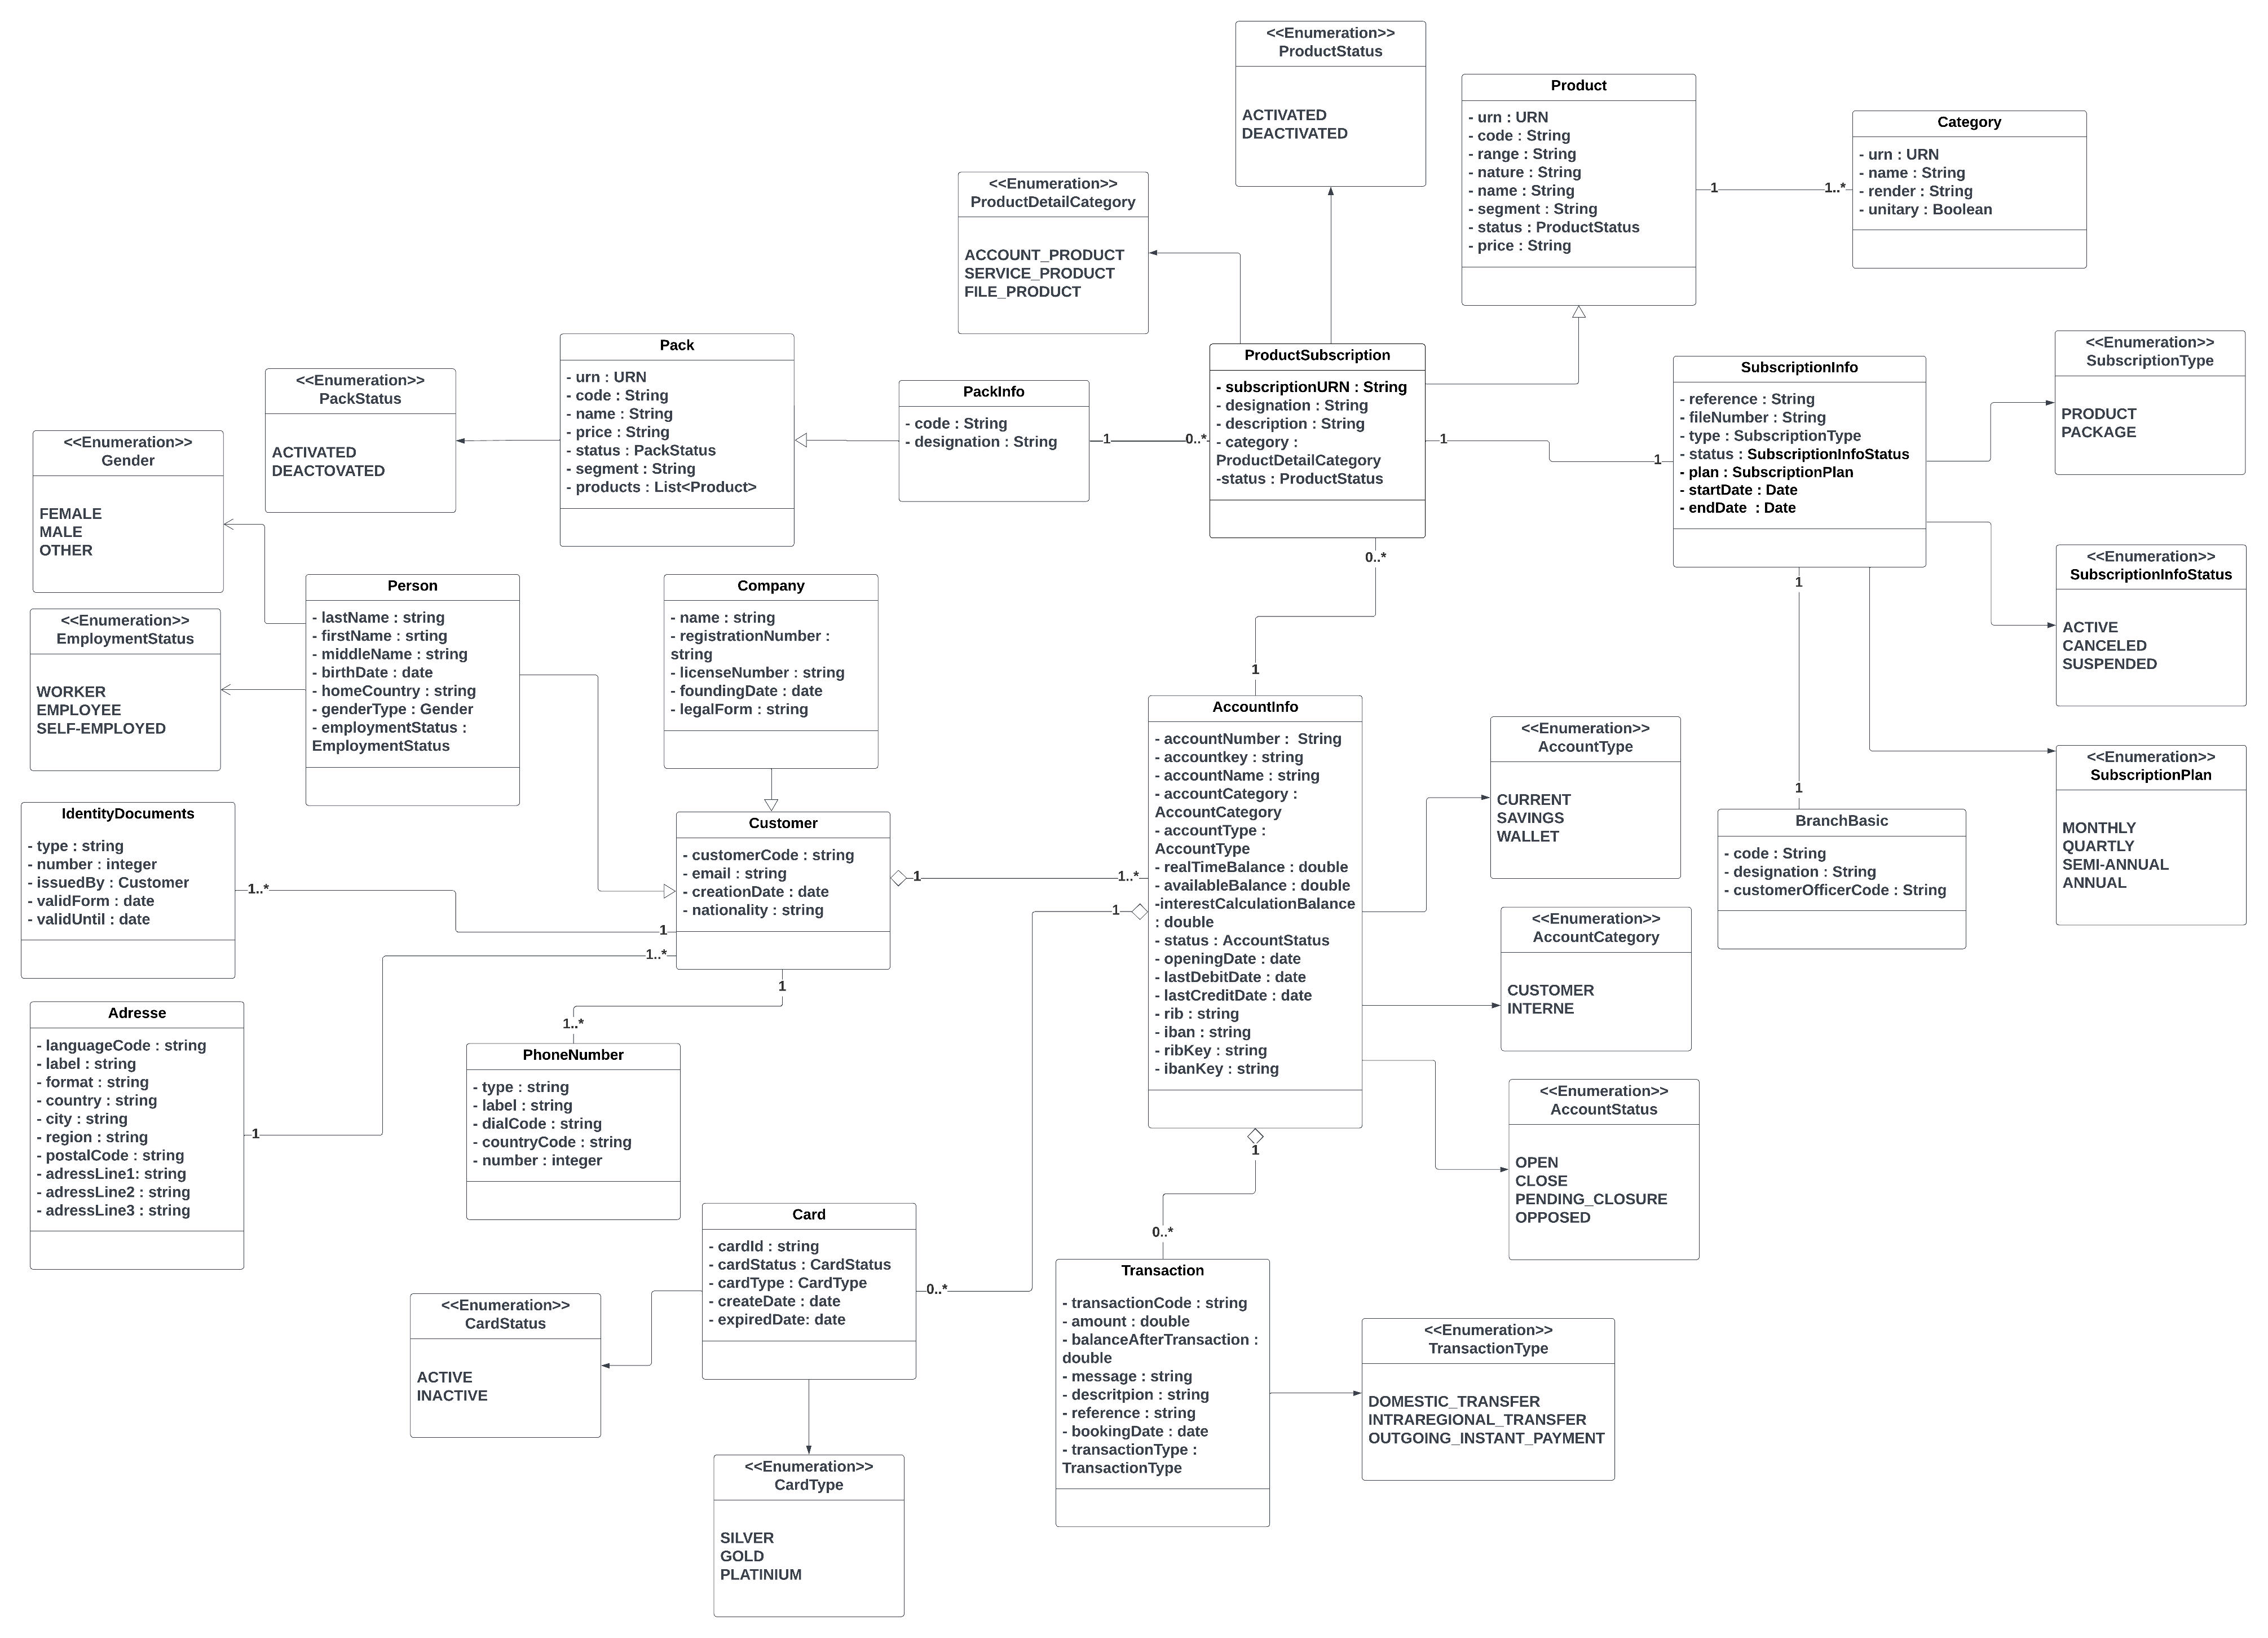
\includegraphics[width=16cm]{images/conception/diagramme_classe.png}
    \caption{Diagramme de classe}
\end{figure}

\section{Diagrammes de séquences}
\subsection{Scénario de consultation des cartes}
\begin{figure}[!h]
    \centering %
        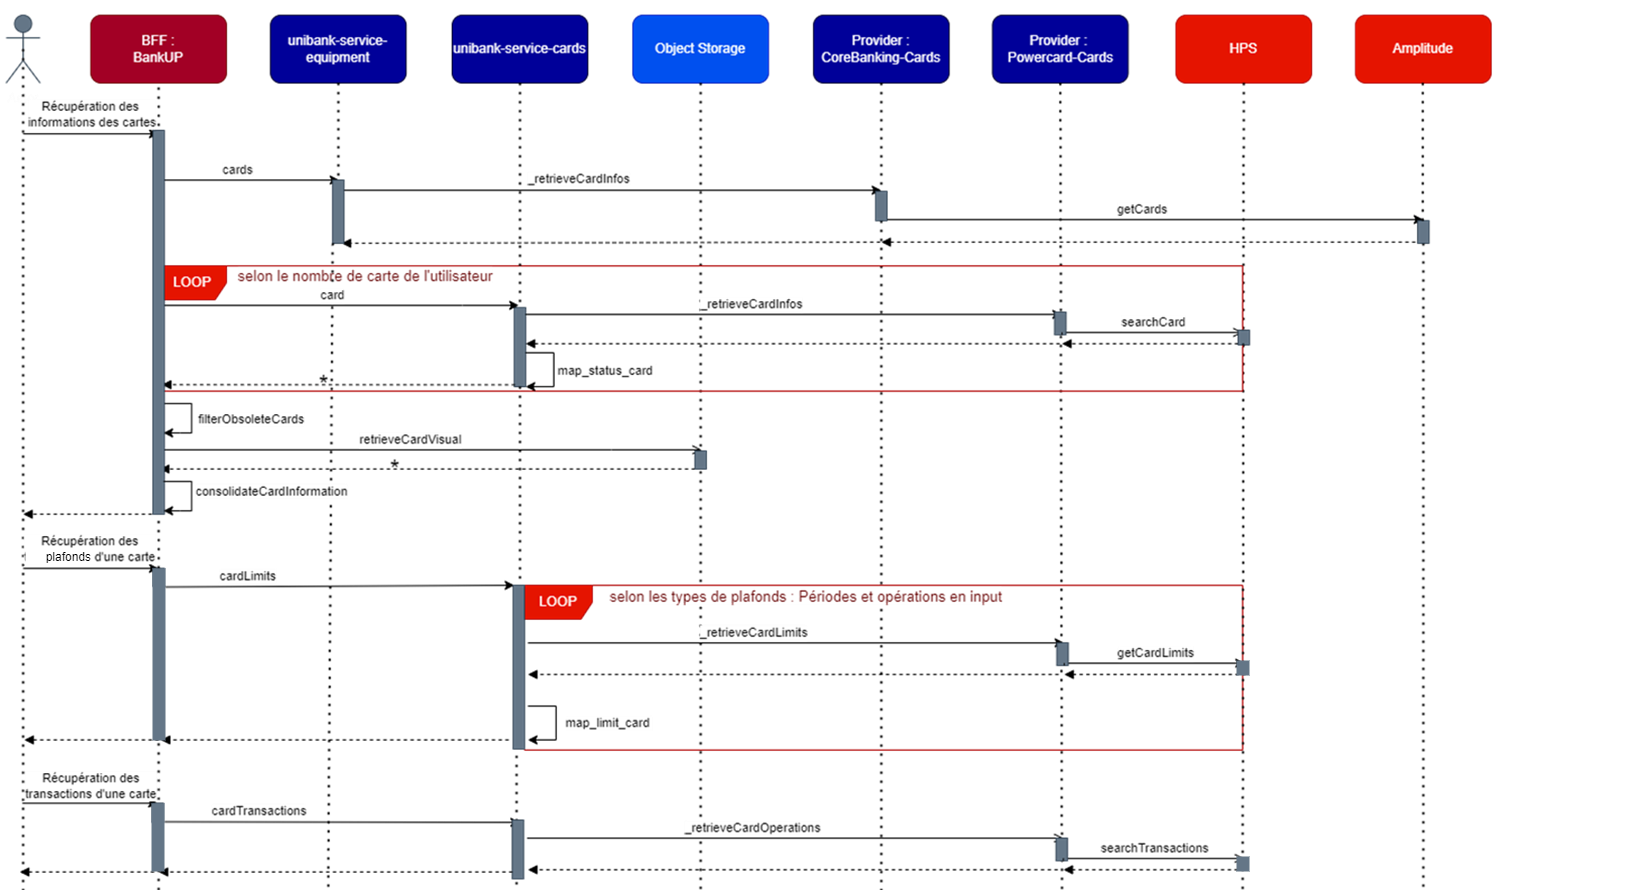
\includegraphics[width=14cm]{images/conception/sequence_cards2.png}
    \caption{Diagramme de séquence d'affichage des cartes, des plafonds et des transactions}
\end{figure}
 
Le diagramme de séquence illustre le scénario de consultation des cartes dans l'interface SG CONNECT. L'utilisateur initie la demande de récupération des informations des cartes via l'interface utilisateur. Pour obtenir les cartes, l'application utilise le service "Unibank Service Equipment" qui agit comme un pont entre l'interface utilisateur et le système bancaire central. Ensuite, le provider "Corebanking-cards" est sollicité pour obtenir les informations spécifiques liées à chaque carte. Cela se fait en utilisant l'API "getCards" fournie par le système bancaire central et en passant par le connecteur "Amplitude" qui assure la communication entre l'application et le système bancaire.\\
Une fois que les informations des cartes sont récupérées, l'application effectue un loop sur le nombre de cartes obtenues. Pendant ce processus, les statuts des cartes sont analysés et adaptés si nécessaire pour répondre aux exigences de l'équipe front-end. Plus précisément, les cartes obsolètes sont filtrées et exclues du résultat final.\\
Une fois les cartes filtrées, l'application peut visualiser et afficher les cartes du client dans l'interface SG CONNECT. Cette étape permet à l'utilisateur de consulter les détails et les informations relatives à chaque carte monétique.\\

Dans le scénario de récupération des plafonds des cartes, l'utilisateur initie la demande via l'interface front du SG CONNECT. Étant donné que nous avons déjà passé par l'étape précédente de récupération des cartes, nous pouvons passer directement à la récupération des plafonds.\\
L'application effectue un loop dans le service "Unibank Service Cards" en fonction du type de plafond, des périodes et des opérations spécifiées par l'utilisateur. En utilisant le provider "Powercard-cards" et l'API "getCardLimits" sur HPS, les plafonds des cartes sont récupérés.\\
Cependant, les données des plafonds peuvent être présentées de manière inhabituelle ou nécessiter une adaptation pour répondre aux besoins de l'application. Par conséquent, un mapping des données est effectué afin de les rendre compatibles avec le format et les exigences de l'interface utilisateur. Cette étape d'adaptation permet d'obtenir les plafonds des cartes dans un format approprié qui sont visualiser et afficher dans l'interface SG CONNECT.\\

Dans le scénario de récupération des transactions liées aux cartes, l'utilisateur initie la demande après avoir déjà obtenu les données des cartes. La demande est ensuite transmise au service "Unibank Service Cards", qui interagit avec le provider "Powercard-cards". En utilisant l'API "searchTransactions" sur HPS, les transactions liées aux cartes sont récupérées.\\
Le processus de récupération des transactions est relativement simple. Après l'initialisation de la demande par l'utilisateur, les étapes suivantes consistent en une séquence de requêtes et de récupération de données. L'interaction entre les différents composants de l'application permet d'obtenir les transactions spécifiques aux cartes sélectionnées.\\
Une fois les transactions récupérées, elles sont affichées à l'utilisateur, lui permettant ainsi de visualiser et de consulter les détails des transactions associées à ses cartes.

\newpage
\subsection{Scénario de consultation des produits}
\begin{figure}[!h]
    \centering %
        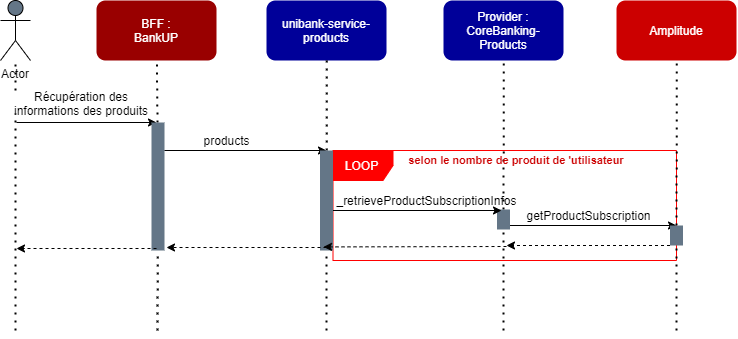
\includegraphics[width=14cm]{images/conception/sequence_products.png}
    \caption{Diagramme de séquence de consultation des produits}
\end{figure}
Dans le scénario de consultation des produits souscrits, l'utilisateur initie la demande de récupération des informations relatives aux produits auxquels il est souscrit. La demande est envoyée vers le service "Unibank Service Products", qui effectue un parcours (loop) pour récupérer tous les produits associés à l'utilisateur via le provider "Corebanking-Products".\\
En utilisant l'API "getProductsSubscription" sur Amplitude, les informations détaillées des produits sont obtenues. Une fois récupérées, ces informations sont affichées à l'utilisateur, lui permettant ainsi de visualiser et de consulter les produits auxquels il est souscrit.
\newpage

\subsection{Scénario de souscription à un produit}
\begin{figure}[!h]
    \centering %
        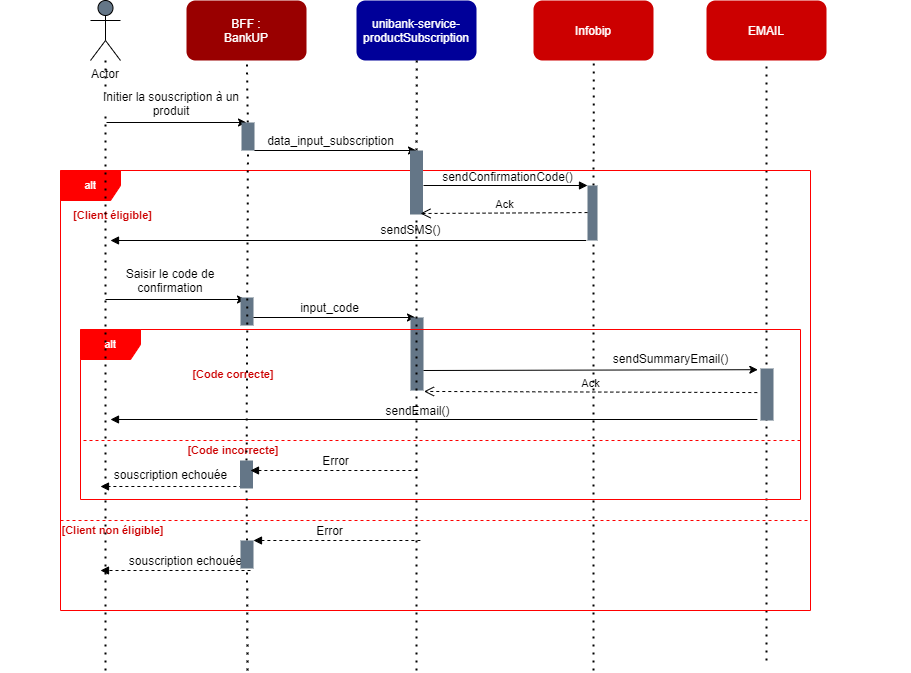
\includegraphics[width=14cm]{images/conception/sequence_souscription.png}
    \caption{Diagramme de séquence de souscription à un produit}
\end{figure}
Dans le scénario de souscription à un produit, l'utilisateur initie la souscription en fournissant certaines informations via l'interface utilisateur de SG CONNECT. Ces informations sont transmises au service "Unibank Service Product Subscription".\\
Si le client est éligible à la souscription, une demande est envoyée à "Infobip" pour l'envoi d'un code de confirmation par SMS. Le code est ensuite envoyé à l'utilisateur qui le saisit dans l'interface utilisateur de SG CONNECT.\\
Le code de confirmation est ensuite vérifié par le service "Unibank Service Product Subscription". Si le code est correct, une demande est envoyée au service "EMAIL" pour l'envoi d'un e-mail récapitulatif de la souscription à l'utilisateur. L'e-mail est alors envoyé à l'utilisateur avec les détails de sa souscription.\\
En revanche, si le code de confirmation est incorrect, le service "Unibank Service Product Subscription" renvoie une erreur qui est affichée à l'utilisateur via l'interface utilisateur de SG CONNECT. De même, si le client n'est pas éligible à la souscription, une erreur est renvoyée par le service vers l'interface utilisateur de SG CONNECT pour être affichée à l'utilisateur.

\section{Conclusion}
Au cours de ce chapitre, nous avons examiné en détail l'architecture monorepo du front-end, l'architecture hexagonale pour la logique métier, l'approche technique d'UNIBANK avec les couches du domaine et de l'application, la technique d'authentification/autorisation avec l'utilisation de JWT et l'algorithme RS256, l'approche multitenant pour gérer les différentes filiales, ainsi que le feature flagging pour activer ou désactiver dynamiquement les fonctionnalités et enfin le diagramme de classe et les diagrammes de séquences.\\
Dans le prochain chapitre, nous aborderons la réalisation et la mise en œuvre de notre application.